 \documentclass[onecolumn]{aastex63}
\usepackage{amsmath}
\usepackage{listings}
\usepackage{tensor}

\lstset{frame=tb,
  language=Python,
  showstringspaces=false,
  columns=flexible,
  basicstyle={\small\ttfamily},
  commentstyle={\small\ttfamily},
  breaklines=true,
  breakatwhitespace=true,
  tabsize=4
}

\usepackage[T1]{fontenc}
\newcommand{\vdag}{(v)^\dagger}
\newcommand\aastex{AAS\TeX}
\newcommand\latex{La\TeX}
\shortauthors{McClellan}
\graphicspath{{./}{figures/}}
\begin{document}

\title{Comprehensive Literature Review}
\author{B. Connor McClellan}
\affiliation{University of Virginia}
\keywords{}

\tableofcontents

% ------- SAMPLE PAPER ------- %
\vspace{1cm}
\hrule
\vspace{1cm}

\section{Sample Paper Title}
\begin{centering}

\cite{sample2020}

\end{centering}

% Uncomment the sections below as you add them

%\subsection{Background}
%%% What are things I learned in order to understand this paper?

%\subsection{Scientific Purpose}
%%% What is the science question addressed by the paper?

%\subsection{Methods}
%%% What is the method used to address the science question?

%\subsection{Citeable Results}
%%% A list of citeable results in the paper
%\begin{itemize}
%    \item
%\end{itemize}
%\subsection{Derivations}
%%% Derivations of any critical equations that appear in the paper

%\subsection{Discussion and Concerns}
%%% Are there any red flags?

%\subsection{Personal Relevance}
%%% Place the work into a familiar context. How is the discussion in the paper related to your own research interests and experience?

%\subsection{Summary}
%%% Reread the abstract, and offer summarizing commentary.
% --------------------------- %

\vspace{1cm}
\hrule
\vspace{1cm}

\section{A Unified Model for Tidal Disruption Events}
\begin{centering}

\cite{dai2018}

\end{centering}

% Uncomment the sections below as you add them

%\subsection{Background}
%%% What are things I learned in order to understand this paper?

%\subsection{Scientific Purpose}
To study the super-Eddington compact disk phase expected in tidal disruption events by using both GRRMHD and Monte Carlo radiative transfer.

%\subsection{Methods}
%%% What is the method used to address the science question?

%\subsection{Citeable Results}
%%% A list of citeable results in the paper
%\begin{itemize}
%    \item
%\end{itemize}
%\subsection{Derivations}
%%% Derivations of any critical equations that appear in the paper

%\subsection{Discussion and Concerns}
%%% Are there any red flags?

%\subsection{Personal Relevance}
%%% Place the work into a familiar context. How is the discussion in the paper related to your own research interests and experience?

%\subsection{Summary}
%%% Reread the abstract, and offer summarizing commentary.


\vspace{1cm}
\hrule
\vspace{1cm}

\section{The Transfer of Resonance-Line Radiation in Static Astrophysical Media}
\begin{centering}

\cite{neufeld1990}

\end{centering}

% Uncomment the sections below as you add them

\subsection{Background}
%% What are things I learned in order to understand this paper?
\textbf{Resonance line}: A spectral line caused by an electron jumping between the ground state and the first energy level in an atom or ion. It is the longest-wavelength line produced by a jump to or from the ground state \citep{ADictionaryofAstronomy}.

The transfer of Ly$\alpha$ radiation is one of the most common mechanisms by which warm astrophysical gas can cool. The Ly$\alpha$ line carries much of the energy radiated by photoionized regions and by interstellar shocks, making it especially luminous in active star-forming regions.

Ly$\alpha$ radiation is frequently scattered by H atoms in the ground state, since it is a resonance line. 

\subsection{Scientific Purpose}
%% What is the science question addressed by the paper?
This paper presents an analytic solution for the mean intensity of resonance-line radiation within an absorbing medium. This solution is valid and agrees with numerical results, provided the medium has large scattering optical depth but low density. The radiation transfer equation takes a second-order, linear partial differential form.

%\subsection{Methods}
%%% What is the method used to address the science question?

%\subsection{Citeable Results}
%%% A list of citeable results in the paper
%\begin{itemize}
%    \item
%\end{itemize}
%\subsection{Derivations}
%%% Derivations of any critical equations that appear in the paper

%\subsection{Discussion and Concerns}
%%% Are there any red flags?

%\subsection{Personal Relevance}
%%% Place the work into a familiar context. How is the discussion in the paper related to your own research interests and experience?

%\subsection{Summary}
%%% Reread the abstract, and offer summarizing commentary.
% --------------------------- %


\vspace{1cm}
\hrule
\vspace{1cm}

\section{The Scattering of Resonance-Line Radiation in the Limit of Large Optical Depth}
\begin{centering}

\cite{harrington1973}

\end{centering}

% Uncomment the sections below as you add them

%\subsection{Background}
%%% What are things I learned in order to understand this paper?

\subsection{Scientific Purpose}
%% What is the science question addressed by the paper?
It is shown that resonance-line radiation transfer in low-density, optically-thick media can be described by the Poisson equation. The mean number of scatterings for escape are calculated, as well as the center and surface line profiles.

\subsection{Methods}
%% What is the method used to address the science question?
The condition for this analytic solution is that the optical depth is so large, the transfer problem is dominated by the redistribution of radiation in the damping wings of the line. Modeling redistribution as a diffusion in frequency space naturally leads to a partial differential equation which turns out to be the Poisson equation. The resulting analytic solution is valid in the limit of large optical depth and matches well to numerical results.

%\subsection{Citeable Results}
%%% A list of citeable results in the paper
%\begin{itemize}
%    \item
%\end{itemize}
\subsection{Derivations}
%%% Derivations of any critical equations that appear in the paper

\begin{equation} \label{harrington1}
    \frac{1}{3\phi^2(x)}\frac{d^2J(\tau, x)}{d\tau^2} = J(\tau, x) - (1-\epsilon)\int_{-\infty}^{\infty}J(\tau, x')q(x, x')dx' - \frac{G(\tau)}{4\pi}
\end{equation}

The general redistribution function, $q(x, x') = R_{II-A}(x, x')/\phi (x)$, is expanded according to \cite{1971JQSRT..11.1365A}. Notably, they define the integrated complementary error function as 

\begin{equation}
    \mathrm{ierfc}(z) \equiv \int_z^{\infty} \mathrm{erfc}(t) dt = \frac{1}{\sqrt{\pi}} e^{-z^2} - z\  \mathrm{erfc}(z)
\end{equation}

The first term in the expansion given by can apparently be neglected in the line wings, so the redistribution function evaluates to 

\begin{equation}
    q(x, x') = \frac{x^2}{s^2} \mathrm{ierfc}(|r|) \approx \left(1+2\frac{r}{x}\right)\mathrm{ierfc(|r|)}
\end{equation}

with $r=(x-x')/2$ and $s=(x+x')/2$, and using the binomial approximation to obtain $x^2/s^2 = (r+s)^2/s^2 = (1+r/s)^2 \approx 1 + 2r/s \approx 1 + 2r/x$. The last step in this approximation comes from the fact that as long as $|x-x'|\ll 1$, $s \approx x$. Note that $1 + 2r/x = 2 - x'/x$.

The $J(x')$ term in the integral in Eq. \ref{harrington1} is then expanded in a Taylor series about $x$.

\begin{equation}
    J(x') \approx J(x) + \frac{dJ(x)}{dx}(x' - x) + \frac{1}{2}\frac{d^2J(x)}{dx^2}(x'-x)^2 + ...
\end{equation}

Thus, the integral becomes

\begin{equation}
    \int_{-\infty}^{\infty}i\ \mathrm{erfc}\left(\frac{|x-x'|}{2}\right)\left(2-\frac{x'}{x}\right)\left[J(x) + \frac{dJ(x)}{dx}(x' - x) + \frac{1}{2}\frac{d^2J(x)}{dx^2}(x'-x)^2 + ...\right] dx'
\end{equation}

Changing variables to $r$, we have

\begin{equation}
    \int_{-\infty}^{\infty}-2i\ \mathrm{erfc}\left(|r|\right)\left(1+2\frac{r}{x}\right)\left[J(x) - 2\frac{dJ(x)}{dx}r + 2\frac{d^2J(x)}{dx^2}r^2 + ...\right] dr
\end{equation}

All $\mathrm{erfc}(|r|)$ terms integrate to $2/\sqrt{\pi}$, while $r\ \mathrm{erfc}(|r|)$ terms (and all others which are odd functions in $r$) evaluate to zero. The $r^2\ \mathrm{erfc}(|r|)$ terms evaluate to $2/(3\sqrt{\pi})$. Therefore, upon evaluating the integral, we are left with

\begin{equation}
    \begin{split}
       -2i\int_{-\infty}^{\infty}&\ \left[J(x)\ \mathrm{erfc}\left(|r|\right) + \left(\frac{2J(x)}{x} - 2\frac{dJ(x)}{dx}\right) r\ \mathrm{erfc}\left(|r|\right) + \left(-\frac{4}{x}\frac{dJ(x)}{dx} + 2\frac{d^2 J(x)}{dx^2}\right)r^2\ \mathrm{erfc}\left(|r|\right) + ...\right]dr \\
       &= -2i \left[\frac{2}{\sqrt{\pi}} J(x) + \frac{2}{3\sqrt{\pi}}\left(-\frac{4}{x}\frac{dJ(x)}{dx} + 2\frac{d^2 J(x)}{dx^2}\right)\right] \\
      &= \frac{-4i}{\sqrt{\pi}} \left[J(x) + \frac{4}{3}\left(-\frac{1}{x}\frac{dJ(x)}{dx} + \frac{1}{2}\frac{d^2 J(x)}{dx^2}\right)\right] \\
   \end{split}
\end{equation}

This result is problematic, since there should be no reason for it to be imaginary. The issue is with Harrington's introduction of $q(x, x')$ as an imaginary number. This, along with the complementary error function, creates additional factors of $1/\sqrt{\pi}$ and returns an imaginary result.

\subsection{Discussion and Concerns}
%% Are there any red flags?

The redistribution function should never be imaginary, yet in the early steps of Harrington's derivation, an integral over an imaginary function to obtain the second order differential equation inexplicably yields a well-behaved, real expansion of $J(x)$ that fits neatly into the equation.

%\subsection{Personal Relevance}
%%% Place the work into a familiar context. How is the discussion in the paper related to your own research interests and experience?

%\subsection{Summary}
%%% Reread the abstract, and offer summarizing commentary.
% --------------------------- %

\vspace{1cm}
\hrule
\vspace{1cm}

\section{ Non-coherent scattering: I. The redistribution function with Doppler broadening}
\begin{centering}

\cite{hummer1962}

\end{centering}

% Uncomment the sections below as you add them

%\subsection{Background}
%%% What are things I learned in order to understand this paper?

\subsection{Scientific Purpose}
%% What is the science question addressed by the paper?

This paper derives the redistribution in frequency of radiation scattered from moving atoms, examining how different circumstances affect the types of scattering which occur in the atom's rest frame. 

\subsection{Methods}
%%% What is the method used to address the science question?

The redistribution function is derived by boosting to the atom's rest frame, where the photon frequency $\nu$ becomes $\xi = \nu - \nu_0 \mathbf{n}\cdot \mathbf{v}/c$. Then, the probability of a photon $(\xi, \mathbf{n})$ being absorbed and re-emitted as a photon $(\xi', \mathbf{n}')$ is calculated using the absorption probability $f(\xi)$ and phase function $g(\mathbf{n}, \mathbf{n}')$ along with the redistribution function $p(\xi, \xi')$ in the atom's rest frame. Then, to obtain $R_v(\nu, \mathbf{n}; \nu', \mathbf{n}')$, we boost back into the lab frame.

%\subsection{Citeable Results}
%%% A list of citeable results in the paper
%\begin{itemize}
%    \item
%\end{itemize}
\subsection{Derivations}
%% Derivations of any critical equations that appear in the paper

Case II-B:

\begin{equation}
    R_{\textrm{II-B}}(x, x') = \frac{3\pi^{-3/2}}{8}\sigma \int_{\frac{1}{2}|\bar{x} - \underset{\bar{}}{x}|}^{\infty} e^{-u^2}
    \int_{\bar{x}-u}^{\underset{\bar{}}{x}+u}\left[3 - \left(\frac{x-t}{u}\right)^2 - \left(\frac{x'-t}{u}\right)^2 + 3\left(\frac{x-t}{u}\right)^2\left(\frac{x'-t}{u}\right)^2\right]\frac{dt\ du}{t^2 + \sigma^2}
\end{equation}

This describes the integrated redistribution function in the radiation-damped dipole scattering case, where 

\begin{equation}
    x = \frac{\nu - \nu_0}{\Delta}
\end{equation}

and $\Delta = \nu_0 \sqrt{2kT/Mc^2}$ (Doppler width).
%\subsection{Discussion and Concerns}
%%% Are there any red flags?

%\subsection{Personal Relevance}
%%% Place the work into a familiar context. How is the discussion in the paper related to your own research interests and experience?

%\subsection{Summary}
%%% Reread the abstract, and offer summarizing commentary.
% --------------------------- %


\vspace{1cm}
\hrule
\vspace{1cm}

\section{Physics of Ly$\alpha$ Radiative Transfer}
\begin{centering}

\cite{dijkstra2017}

\end{centering}

% Uncomment the sections below as you add them

%% What are things I learned in order to understand this paper?

\subsection{Cosmology}

Dark matter can be modeled as a pressureless fluid that interacts only graviationally with baryonic matter. Dark energy is represented by a negative pressure that contributes to the accelerating expansion of the universe.

\subsection{Ly$\alpha$ Emission}
Ly$\alpha$ is a \textbf{resonance line}. The scattering cross section increases sharply toward line center, so photons with this frequency are more likely to be scattered rather than emitted towards the observer. Once scattered away from line center by interacting with moving gas particles, the scattering opacity decreases. This explains the double-peaked emission feature associated with Ly$\alpha$. Typical astrophysical environments are optically thick to Ly$\alpha$, so full radiative transfer is needed to understand Ly$\alpha$ emitting sources.

The Lyman series of spectral lines involves all electron transitions between $n \ge 2$ to $n = 1$. The first of these transitions, $n = 2$ to $n = 1$, is Ly$\alpha$. Selection rules dictate that only transitions of the form $|\Delta l| = 1$ are allowed --- therefore, a transition from a $2s$ orbital to a $1s$ orbital is impossible unless two photons are emitted.

\subsection{Collisional Excitation} A hydrogen atom can become excited via collision between an electron and the atom, in which kinetic energy of a free electron is expended to excite the atom. Since the electron's kinetic energy is associated with the thermal energy of the gas, emitting Ly$\alpha$ has the effect of cooling the gas.

The efficiency of this process depends on the relative velocity of the two particles, and the number density of each species. The total Ly$\alpha$ production rate through collisional excitation is 

\begin{equation}
    R_{col}^{Ly\alpha} = n_e n_h q_{1s2p}\ \textrm{cm}^{-3} \textrm{s}^{-1}
\end{equation}

where the rate coefficient depends on the velocity averaged collision strength. The cooling rate per unit volume, which depends on the ionization state of the gas, ends up being a function of temperature only.

\subsection{Recombination} When a free proton and electron recombine, the electron can be left in any quantum state. Radiative cascades to the ground state can then produce a Ly$\alpha$ photon. The probability of this emission can be quantified by a weighted sum over all of the quantum states in the radiative cascade.

\textbf{Case A recombination} takes place in a medium that is optically thin at all photon frequencies. Direct recombination to the ground state is allowed.

\textbf{Case B recombination} takes place in a medium that is opaque to all Lyman series photons and to ionizing photons that were emitted following direct recombination into the ground state. Photons that are produced are immediately absorbed by a neighboring H atom.

\subsection{Ly$\alpha$ Scattering Cross-Section}

By evaluating the Ly$\alpha$ cross-section, we can determine which astrophysical sources are optically thick to this radiation. Start with the Thomson cross section. Suppose a free electron interacts with an incoming electromagnetic wave. 

\noindent Amplitude of electric field:
\begin{equation}
    E(t) = E_0 \sin{\omega t}
\end{equation}

\noindent Acceleration experienced by electron:
\begin{equation}
    \alpha(t) = \frac{q|E(t)|}{m_e}
\end{equation}

\noindent Electron's radiated power (Larmor formula):
\begin{equation}
    P(t) = \frac{2}{3}\frac{q^2\alpha^2}{c^3}
\end{equation}

\begin{equation}
    \langle P \rangle = \frac{q^4E_0^2}{3c^3m_e^2}
\end{equation}

\noindent Electromagnetic flux (Poynting's Theorem):
\begin{equation}
    F = c\frac{\mathbf{E} \times \mathbf{B}}{4\pi} = \frac{cE_0^2 \langle \sin^2 (\omega t)\rangle}{4\pi} = \frac{cE_0^2}{8\pi}
\end{equation}

\noindent The Thomson scattering cross-section is the ratio of the total radiated power to the total incident flux. 

\begin{equation}
    \sigma_T = \frac{q^4 E_0^2}{3c^3m_e^2} \frac{8\pi}{cE_0^2} = \frac{8\pi}{3}\frac{q^4}{c^4m_e^2} = \frac{8\pi}{3}r_e^2
\end{equation}

where $r_e = q^2 / (m_ec^2)  = 2.8 \times 10^{-13}$ cm is the classical electron radius. The re-emitted radiation is strongly angle dependent, and can be integrated over to obtain

\begin{equation}
    \frac{P(\mu)}{F} = \frac{\sigma_T P(\mu)}{4\pi}
\end{equation}

 \noindent with
 
\begin{equation}
    P(\mu) = \frac{3}{4}(1 + \mu^2)
\end{equation}

\noindent for dipole or Rayleigh scattering, and 

\begin{equation}
    P(\mu) = 1
\end{equation}

for isotropic scattering. Here, $\mu = \cos{\theta}$ and $\theta$ is the angle between the incoming and outgoing electromagnetic radiation.

If, instead, a bound electron interacts with an incoming electromagnetic wave, a Lorentzian cross-section is derived by treating the electron as a damped harmonic oscillator. Following the same derivation as above with a different equation of motion, we arrive at 

\begin{equation}
    \sigma(\omega) = \frac{\sigma_T}{4\omega_0^2} \frac{\omega^4}{(\omega-\omega_0)^2 + \Gamma^2/4}
\end{equation}

This equation exhibits resonant behavior at the natural frequency $\omega = \omega_0$, at which the cross section increases sharply. Otherise, the $\omega^4$ dependence suggests the atom is more efficient at scattering highly energetic radiation.

When treated quantum-mechanically, the parameter $\Gamma$ is reduced by a factor called the oscillator strength. Additionally, a functional form of the Ly$\alpha$ cross-section doesn't exist, since the contributions to the cross-section from higher-order Lyman-series transitions must be taken into account far from resonance.

Each atom in a gas has its own velocity, so a photon of fixed frequency $\nu$ will appear Doppler boosted to a slightly different frequency for each atom in the gas. Convolution of the single-atom cross-section with the gas's velocity distribution yields the total Ly$\alpha$ cross-section for the gas. This takes the form of a Voigt profile. The Ly$\alpha$ cross-section is 11 orders of magnitude larger than the Thomson cross-section, meaning radiation is scattered 11 orders of magnitude more efficiently off of bound electrons than free electrons when the frequency of the radiation closely matches the natural frequency of the transition.

%\subsection{Scientific Purpose}
%%% What is the science question addressed by the paper?

%\subsection{Methods}
%%% What is the method used to address the science question?

%\subsection{Citeable Results}
%%% A list of citeable results in the paper
%\begin{itemize}
%    \item
%\end{itemize}
%\subsection{Derivations}
%%% Derivations of any critical equations that appear in the paper

%\subsection{Discussion and Concerns}
%%% Are there any red flags?

%\subsection{Personal Relevance}
%%% Place the work into a familiar context. How is the discussion in the paper related to your own research interests and experience?

%\subsection{Summary}
%%% Reread the abstract, and offer summarizing commentary.
% --------------------------- %


\vspace{1cm}
\hrule
\vspace{1cm}

\section{A giant comet-like cloud of hydrogen escaping the warm Neptune-mass exoplanet GJ 436b}
\begin{centering}

\cite{ehrenreich2015}

\end{centering}

% Uncomment the sections below as you add them

%\subsection{Background}
%%% What are things I learned in order to understand this paper?

\subsection{Scientific Purpose}
%% What is the science question addressed by the paper?
This paper reports ultraviolet transit depths of 56\% for the exoplanet GJ 436b, indicating the presence of a large exospheric hydrogen cloud.

%\subsection{Methods}
%%% What is the method used to address the science question?

\subsection{Citeable Results}
%% A list of citeable results in the paper
\begin{itemize}
    \item The most notable absorption occurs in the blue wing of the Ly-$\alpha$ line
    \item Over half (56.3\%) of the stellar disk is eclipsed, and a total Ly-$\alpha$ eclipse would have been possible for a central transit
    \item Stellar radiation pressure counterbalances approximately 70\% of the star's gravitational pull on escaping atoms
\end{itemize}

%\subsection{Derivations}
%%% Derivations of any critical equations that appear in the paper

%\subsection{Discussion and Concerns}
%%% Are there any red flags?

%\subsection{Personal Relevance}
%%% Place the work into a familiar context. How is the discussion in the paper related to your own research interests and experience?

%\subsection{Summary}
%%% Reread the abstract, and offer summarizing commentary.
% --------------------------- %

\vspace{1cm}
\hrule
\vspace{1cm}

\section{An extended upper atmosphere around the extrasolar planet HD209458b}
\begin{centering}

\cite{vidal-madjar2003}

\end{centering}

% Uncomment the sections below as you add them

\subsection{Background}
%% What are things I learned in order to understand this paper?

The Ly-$\alpha$ line is a spectral line of single-electron ions (or hydrogen) that is associated with the $n=2$ / $n=1$ transition. In hydrogen, its wavelength is 1215.67 \r{A}. Deuterium is shifted slightly toward the blue, which can explain some of the blue absorption.

\subsection{Scientific Purpose}
%% What is the science question addressed by the paper?
This paper reports detection of atomic hydrogen (H) absorption in the stellar Ly-$\alpha$ line during three transits of the exoplanet HD209458b. The planet's radius and mass suggest the absorption takes place beyond the Roche limit (i.e., the absorption is occurring in escaped H atoms).

\subsection{Methods}
%% What is the method used to address the science question?
Observational data was taken from the Space Telescope Imaging Spectrograph (STIS) onboard the Hubble Space Telescope (HST) using the G140M grating to minimize contamination from Earth's Ly-$\alpha$ geocoronal emission. The remaining geocoronal emission was removed by subtracting the sky spectrum from the stellar spectrum (possible because the sky spectrum fulls the entire aperture of the spectrograph). Two separate methods for dark-subtraction were used, both converging at the same result with low systematic errors. 

The Ly-$\alpha$ spectrum of HD209458 is typical --- it has a double-peaked emission feature, since the temperature increase in the lower chromosphere causes an emission line with a central dip due to the high opacity of the abundant hydrogen atoms. 

The three exposures taken outside transits and entirely within transits were each co-added to improve the signal-to-noise ratio. In the transit interval, the Ly-$\alpha$ line is reduced by 15 $\pm$ 4\%. 

HD209458 is a solar-type star, which can vary in chromospheric Ly-$\alpha$ strength. Line strength \textit{in our Sun} was used as a proxy for HD209458, measured using SOHO. With these observations, it was confirmed that on timescales of a few months the Ly-$\alpha$ line strength (`In/Out ratio'') varies by less than 4\%. The observed absorption seen in HD209458 is assumed to be outside of standard chromospheric variation.

The magnitude of absorption is larger than it should be for a planet occulting 1.5\% of the star's visible surface. A maximally-filled Roche lobe would account for only 10\% absorption. The outlying 5\% suggests that hydrogen is escaping the planet's atmosphere. 

A particle model is built accounting for stellar radiation pressure inside and outside the Roche lobe, as well as the planetary and stellar gravity. Ly-$\alpha$ radiation pressure is 0.7 times the stellar gravity, while the escape flux and neutral hydrogen lifetime are treated as free parameters. Due to UV ionization, the neutral hydrogen lifetime is set to be a few hours. 
However, to fully account for the 15\% absorption depth, a more sophisticated treatment is needed. To obtain a more accurate escape flux measurement, the vertical distribution of H atoms up to the Roche limit must be characterized, in which the atmosphere is extended by stellar tidal forces and heating mechanisms. 

\subsection{Citeable Results}
%% A list of citeable results in the paper
\begin{itemize}
    \item Models suggest escaping hydrogen atoms expand in an asymmetric comet-like tail and progressively disappear when moving away from the planet, which is consistent with observations.
    \item The absorption lasts well after the end of the transit due to the large physical size of the evaporating tail
    \item The absorption is blueshifted because of the radiation pressure repelling the atoms away from the star
\end{itemize}

%\subsection{Derivations}
%%% Derivations of any critical equations that appear in the paper

\subsection{Discussion and Concerns}
%% Are there any red flags?
\textbf{Double-peaked emission feature:} I'm a bit unclear on how the temperature increase in the chromosphere can create this specific spectral signature. My best guess is that a Ly-$\alpha$ emission takes place in the chromosphere and is thermally broadened, but the cooler outer layers absorb at the same central wavelength. Since the absorption isn't broadened, the line strength is only diminished at the very center.

\textbf{Chromospheric Ly-$\alpha$ Variation:} Spectral data from the Sun were used as justification that HD209458 couldn't have had natural chromospheric Ly-$\alpha$ variation larger than 4\%. While HD209458 is nearly solar-type, this judgement seems a little weak, and the error in the line strength is probably larger than reported as a result.

%\subsection{Personal Relevance}
%%% Place the work into a familiar context. How is the discussion in the paper related to your own research interests and experience?

\subsection{Summary}
%% Reread the abstract, and offer summarizing commentary.

Mass and radius measurements allow advanced analysis to be done on Ly-$\alpha$ spectral features, as it is possible to discern what fraction of the absorbing atoms are gravitationally bound to the planet. It has been determined observationally that HD209458b is evaporating, producing a streaming tail of escaping hydrogen atoms.

% --------------------------- %


\vspace{1cm}
\hrule
\vspace{1cm}

\section{The Athena++ Adaptive Mesh Refinement Framework: Design and Magnetohydrodynamic Solvers}

\begin{centering}

\cite{stone2020}

\end{centering} 

\subsection{Derivations}

\begin{equation} \label{40b} 
    \nabla_\mu T\indices{^\mu_\nu} = 0
\end{equation}

Eq. \ref{40b}, which is Eq. 40b in \cite{stone2020}, is an equation of general relativistic magnetohydrodynamics, which takes the form of a four-momentum conservation law. The equation corresponding to the zeroth component of the four-momentum describes conservation of energy, and the remaining three indices describe conservation of 3-momentum. In this derivation, the conservation law will be written in a more useful form which can be solved directly in \texttt{Athena++}.

We start by expanding the covariant derivative in terms of Christoffel symbols.

\begin{equation}
    T\indices{^\mu_{\nu ; \mu}} =  T\indices{^\mu_{\nu , \mu}} + \Gamma \indices{^\mu _{\alpha \mu}} T\indices{^\alpha _\nu} - \Gamma \indices{^\alpha _{\nu \mu}} T\indices{^\mu _\alpha} = 0
\end{equation}

\begin{equation} \label{carriedover}
    T\indices{^\mu_{\nu , \mu}} + \Gamma \indices{^\mu _{\alpha \mu}} T\indices{^\alpha _\nu} = \Gamma \indices{^\alpha _{\nu \mu}} T\indices{^\mu _\alpha}
\end{equation}

The Christoffel symbols can be written in terms of the metric tensor with

\begin{equation} \label{metric_expand}
    \Gamma \indices{^\alpha _{\nu \mu}} = \frac{1}{2}g\indices{^{\alpha \beta}} \left( g\indices{_{\beta \nu , \mu}} + g\indices{_{\beta \mu , \nu}} - g\indices{_{\nu \mu, \beta}} \right)
\end{equation}


\begin{equation} \label{metric_trace}
    \begin{split}
            \Gamma \indices{^\mu _{\alpha \mu}} &= \frac{1}{2}g\indices{^{\mu \beta}} \left( g\indices{_{\beta \alpha , \mu}} + g\indices{_{\beta \mu , \alpha}} - g\indices{_{\alpha \mu, \beta}} \right) \\
            &= \frac{1}{2} g\indices{^{\mu \beta}} \left(g\indices{_{\beta \mu , \alpha}} + 2g\indices{_{\alpha [\beta  , \mu]}} \right) \\
            &= \frac{1}{2} g\indices{^{\mu \beta}} g\indices{_{\mu \beta, \alpha}}
    \end{split}
\end{equation}

since the product of the symmetric tensor $g\indices{^{\mu \beta}}$ with the antisymmetric tensor $g\indices{_{\alpha [\beta  , \mu]}}$ yields zero. The partial derivative of the trace of the metric tensor, $g\indices{_{, \alpha}}$, can be written 
\begin{equation}
    g\indices{_{, \alpha}} = g\indices{^{\mu \beta}} g\indices{_{\mu \beta, \alpha}} g
\end{equation}

and therefore, by comparison with Eq. \ref{metric_trace}, we have

\begin{equation} \label{sqrtnegative}
    \Gamma \indices{^\mu _{\alpha \mu}} = \frac{1}{2} \frac{g\indices{_{, \alpha}}}{g} = \frac{\left(\sqrt{-g}\right)\indices{_{, \alpha}}}{\sqrt{-g}}
\end{equation}

where the last equality can be confirmed via the chain rule. Substituting Eqs. \ref{metric_expand} and \ref{sqrtnegative} into Eq. \ref{carriedover}, we obtain

\begin{equation} \label{writtenallout}
    T\indices{^\mu _{\nu, \mu}} + \frac{\left(\sqrt{-g}\right)\indices{_{, \alpha}}}{\sqrt{-g}} T\indices{^\alpha _\nu} = \frac{1}{2}g\indices{^{\alpha \beta}} \left( g\indices{_{\beta \nu , \mu}} + g\indices{_{\beta \mu , \nu}} - g\indices{_{\nu \mu, \beta}} \right) T\indices{^\mu _\alpha}
\end{equation}

Using $g\indices{^{\alpha \beta}}$ to raise the second index on $T\indices{^\mu _\alpha}$ in Eq. \ref{writtenallout}, we obtain a product between a symmetric tensor $T\indices{^\mu ^\beta}$ and an antisymmetric tensor $g\indices{_{\nu [\beta, \mu]}}$, which yields zero.

\begin{equation}
    \begin{split}
    T\indices{^\mu _{\nu, \mu}} + \frac{\left(\sqrt{-g}\right)\indices{_{, \alpha}}}{\sqrt{-g}} T\indices{^\alpha _\nu} &= \frac{1}{2}g\indices{^{\beta \alpha}} T\indices{^\mu _\alpha} \left(g\indices{_{\beta \mu , \nu}} + 2 g\indices{_{\nu [\beta, \mu]}} \right) \\
    &= \frac{1}{2}T\indices{^\mu ^\beta} \left(g\indices{_{\beta \mu , \nu}} + 2 g\indices{_{\nu [\beta, \mu]}} \right) \\
    &= \frac{1}{2}T\indices{^\mu ^\beta} g\indices{_{\mu \beta, \nu}} \\
    \end{split}
\end{equation}

We change the dummy index $\mu \rightarrow \alpha$ on both sides, and change the free index $\nu \rightarrow \mu$. With these modifications, multiplied through by $\sqrt{-g}$,  Eq. \ref{writtenallout} simplifies to 

\begin{equation} \label{writtenallout_simplified}
    \sqrt{-g}\ T\indices{^\alpha _{\mu, \alpha}} + \left(\sqrt{-g}\right)\indices{_{, \alpha}} T\indices{^\alpha _\mu} = \frac{1}{2} \sqrt{-g}\ T\indices{^\alpha ^\beta} g\indices{_{\alpha \beta , \mu}}
\end{equation}

The two terms on the left-hand side can be combined, producing

\begin{equation} \label{writtenallout_simplified}
    \left(\sqrt{-g}\ T\indices{^\alpha _\mu}\right)\indices{_{, \alpha}}  = \frac{1}{2} \sqrt{-g}\ g\indices{_{\alpha \beta , \mu}} T\indices{^\alpha ^\beta} 
\end{equation}

When rewritten in terms of partial derivatives, we obtain 

\begin{equation} \label{writtenallout_simplified}
    \partial\indices{_t}\left(\sqrt{-g}\ T\indices{^0 _\mu}\right) +  \partial\indices{_j}\left(\sqrt{-g}\ T\indices{^j _\mu}\right)= \frac{1}{2} \sqrt{-g}\ \left(\partial\indices{_\mu} g\indices{_{\alpha \beta}}\right)T\indices{^\alpha ^\beta} 
\end{equation}

which is Eq. 42b in \cite{stone2020}.

\vspace{1cm}
\hrule
\vspace{1cm}

\section{Models of X-Ray Bursters with Radius Expansion}

\begin{centering}

\cite{paczynski1983}

\end{centering} 


\subsection{Scientific Purpose}
To present a series of models which are kept as simple as possible, but with a careful treatment of certain effects that may be important for neutron star envelope expansion.
\subsection{Methods}
Models were created with a fully general relativistic treatment. The importance of allowing the electron scattering opacity to vary with temperature and density is stressed. The accreted matter was 97\% helium and 3\% magnesium. Only nuclear flashes were calculated, under spherical symmetry and assumed to be in hydrostatic equilibrium for the duration of the burst. All radiation flowing from the burst is due to helium burning within the envelope.

There is a point at which the chemical composition changes at the base. Inner boundary conditions are applied here, assuming that the radius stays constant and the heat flux is zero. This condition is maintained throughout the evolutionary computations that follow. 

When the surface luminosity was low, the outer boundary condition was applied at the outermost mass point at a column depth of 1 g cm$^{-2}$. The opacity is assumed to be constant above this point, and the surface temperature $T_0$ is related to the effective temperature $T_e$ by $2T_0^4 = T_e^4 = F/\sigma$. 

When the surface luminosity approached the Eddington limit, the outer boundary condition was moved to a mass point at 10$^{-16}\ M_\odot$ below the surface. 

\subsection{Citeable Results}
\begin{itemize}
    \item A major expansion of a neutron star envelope is possible if the pressure at the bottom of the envelope is sufficiently high, which implies a high base envelope temperature and density at the peak of the flash
\end{itemize}

\subsection{Discussion and Concerns}
When the electron scattering opacity is mentioned, it is emphasized that it is dependent on both density and temperature. However, what we refer to as ``electron scattering opacity'' is typically just $\kappa_{es} = 0.2(1 + X)$ cm$^2$/ g.

Paczynski uses a formula that approximates tabulated values by Buchler and Yueh (1976). Electron scattering opacity decreases at high temperature due to relativistic electron velocities, and decreases at high density due to electron degeneracy. 

\begin{equation}
    \kappa_{es} = 0.2\left(1 + 2.7 \times 10^{11}\rho T^{-2}\right)^{-1} \times \left[1 + \left(\frac{T}{4.5\times10^8}\right)^{0.86}\right]^{-1}
\end{equation}

%\subsection{Personal Relevance}
%%Place the work into a familiar context. How is the discussion in the paper related to your own research interests and experience?

\subsection{Notable References}
\begin{itemize}
    \item \textbf{Paczynski (1977)} Describes code used in evolutionary calculations for this paper
    \item \textbf{Thorne (1977)} General relativistic stellar structure equations
\end{itemize}
%\subsection{Summary}
%\textcolor{lightgray}{Reread the abstract, and offer summarizing commentary.}


\section{Super-Eddington Winds from Type I X-ray Bursts}
\begin{centering}

\cite{yu2018}

\end{centering}

\subsection{Background}
\begin{itemize}
    \item The temperature of the emitting area of the photosphere decreases below 1 keV, which means X-ray detectors like PCA on the RXTE lose signal at this point in the burst. NICER does not have this issue since it remains sensitive down to 0.2 keV.
    \item An optically thick, radiation-driven wind emerges after the burst rise, which can contain ashes of nuclear burning ($^4$He, $^{12}$C, heavy elements A > 40) depending on the ignition depth of the burst.
        \begin{itemize}
            \item The heavy elements can imprint absorption edges and lines on the burst spectra. Inclusion of absorption edges in spectral models can significantly improve the fit of the data. \textbf{(?)}
        \end{itemize}
    \item In the optically thin region of the photosphere, Compton scattering is important. In the radiative outer shell, the temperature profile is shallow, and the opacity varies only slightly with column depth.
\end{itemize}
\subsection{Scientific Purpose}
The aim of this paper is to model the hydrodynamics of spherically symmetric super-Eddington winds from radius expansion bursts. The new science being done is that the calculations are time-dependent, and have the ability to evaluate whether previous steady-state models are valid or not. 
\subsection{Methods}

The post-He ignition calculation can be separated into two time-dependent stages: the hydrostatic heating stage (burst rise) followed by the hydrodynamic wind phase (PRE).

The hydrostatic burst phase uses nuclear physics calculations in MESA. Pure He accretion is assumed, due to the high luminosity of PREs that ignite in a pure He layer. Local Thermodynamic Equilibrium (LTE) is assumed. The hydrostatic burst rise simulations involve modeling convection using mixing-length theory, for which the top boundary is set at an optical depth of $\tau = 100$ (quite deep, compared with the boundary for the hydrodynamic wind at $\tau = 3$). This boundary is sensible given that the atmospheric evolution is driven entirely by nuclear burning in this phase. A vertical coordinate \textit{y} describes the column depth, which is the integral of the density from some radius \textit{r} outwards to infinity. We have

\begin{equation}
    y \approx \frac{P}{g} \approx \frac{M_r}{4\pi R^2}
\end{equation}

where $P$, $g$, and $M_r$ are the pressure, gravitational acceleration, and mass above $r$.

A note on the simulation notation: calculations were performed for burst ignition at three column depths $(y1, y2, y3) = (0.5, 1.5, 5) \times 10^9$ g cm$^{-2}$, using either a 9-isotope network (n9) or a 21-isotope network (n21).

The hydrodynamic wind phase uses MESA's hydrodynamics solver under the diffusion approximation in local thermodynamic equilibrium. The atmosphere is almost fully radiative at this stage, so mixing-length theory convection is turned off. The radiation is given by

\begin{equation}
    \frac{dT^4}{dr} = \frac{-3\kappa \rho L_{\textrm{rad}}}{4\pi a c r^2}
\end{equation}

The photospheric radius is the location where $L_rad/4\pi r_{\textrm{ph}}^2 = \sigma T^4$. \textbf{The diffusion approximation breaks down above this radius, so this region is not well treated in this paper.} During the wind phase, the mass-loss rate, temperature, density, and optical depth all increase throughout the wind, but the velocity decreases having never exceeded 0.01c. All the wind profiles of the burst models at different ignition depths match closely, since the wind structure is largely dependent on the mass-loss rate. The models have very similar mass-loss rates up until the wind terminates. The duration of the wind phase increase with increasing ignition depth, but the structure is nearly independent from it.

\subsection{Citeable Results}
\begin{itemize}
    \item It takes a few seconds for time-independent conditions to be established in the wind. Since most PREs only last a few seconds, the steady-state assumption is not well satisfied.
    \item During the burst rise, the base temperature rises due to He burning, forming a convective region that extends outward to lower pressure on timescales of milliseconds. This occurs so quickly that the thermal profile in the radiative region is unchanged since before the ignition.
    \item In order to properly account for the driving of the wind, it is necessary to consider the transport of heat by convection and radiative diffusion through the hydrostatic layers between the ignition base and the wind base. 
    \item $L_{Edd} \propto \kappa(T)^{-1} \propto T^{0.86}$. At high temperature (larger column depth), a given luminosity can be sub-Eddington but may become super-Eddington as the radiation diffuses upward into shallower layers.\textbf{ As a result, the base of the wind is initially at small column depth, moves inwards as the deeper layers heat up, and then moves back outward to smaller column depth as the layers cool.}
    \item ${\sim}$30\% of the nuclear energy of the burst goes to unbinding matter from the neutron star surface, independent of ignition depth.
    \item By the time the wind has settled into a steady state at $t=10$ s, it is predominantly composed of heavy-element ashes (50\% $^{48}$Cr). 
\end{itemize}

%\subsection{Discussion and Concerns}
%\textcolor{lightgray}{Are there any red flags?}

\subsection{Personal Relevance}
I aim to simulate the exact same phenomenon as that which is described in this paper. However, Yu and Weinberg state that, although their results are broadly consistent with observations, there are some notable differences. They suspect the differences may be attributed to several simplifying assumptions made, including their neglect of general relativistic effects and a simplified treatement of radiation transfer. \textit{My work will address these differences by performing the simulations in full general relativity with realistic radiation transport} (i.e., non-Newtonian and not under the diffusion approximation).

%\subsection{Summary}
%\textcolor{lightgray}{Reread the abstract, and offer summarizing commentary.}

\vspace{1cm}
\hrule
\vspace{1cm}

\section{The Structure and Appearance of Winds from Supercritical Accretion Disks II: Dynamical Theory of Supercritical Winds}
\begin{centering}

\cite{meier1982}

\end{centering}


\subsection{Background}
\begin{itemize}
    \item A ``supercritical'' wind exists if the total energy generated per unit time exceeds the Eddington limit
    \begin{equation}
        L_{Edd} = \frac{4\pi G M c}{\kappa_{es}}
    \end{equation}
    \item Winds could be driven by supercritical accretion disks, \textbf{inhomogeneous spherical accretion}, or from the surface of the star, if internal nuclear luminosity is super-Eddington
    \item Energy generation time scale:
    \begin{equation}
        t_{gen} = \frac{p_iE_i + P_i}{\dot \epsilon_i}
    \end{equation}
    where $\rho_i$ is the mass density, $E = 3RT/2\mu + 4\pi J/\rho c$ is the total specific energy (gas plus radiation), and $P = \rho R T / \mu + 4\pi K / c$ is the total pressure of the matter at $r_i$.
    \item The trapping radius is where radiation is trapped and the flow is adiabatic. It is found by setting the Eulerian flux of photons advected by the wind equal to the diffusive flux of photons.
    \begin{equation}
        F_a = \rho v E_r + P_r v = -\frac{c}{\kappa_{es} \rho}\frac{dP_r}{dr} = F_\gamma \approx \frac{cP_r}{\kappa_{es}\rho r}
    \end{equation}
\end{itemize}

%\subsection{Scientific Purpose}
%\textcolor{lightgray}{What is the science question addressed by the paper?}
%\subsection{Methods}
%\textcolor{lightgray}{What is the method used to address the science question?}
%\subsection{Citeable Results}
%\begin{itemize}
%    \item \textcolor{lightgray}{A list of citeable results in the paper}
%\end{itemize}
%\subsection{Discussion and Concerns}
%\textcolor{lightgray}{Are there any red flags?}
%\subsection{Personal Relevance}
%\textcolor{lightgray}{Place the work into a familiar context. How is the discussion in the paper related to your own research interests and experience?}
%\subsection{Summary}
%\textcolor{lightgray}{Reread the abstract, and offer summarizing commentary.}

\vspace{1cm}
\hrule
\vspace{1cm}

\section{Super-Eddington Winds from Neutron Stars}
\begin{centering}

\cite{paczynski1990}

\end{centering}


\subsection{Background}
In a degenerate gas, there is sufficiently high density and low temperature such that random thermal motions of particles in the gas no longer supply much pressure. If the gas is ionized, quantum mechanical considerations come into play. The Pauli Exclusion Principle implies that as you add more particles to the system, they must have an energy above all the other particles already there. For a non-degenerate gas, there is enough thermal motion that particles can exist in states that are not packed in close to each other. Quantum effects can be ignored. Degeneracy pressure dominates when $k_b T \ll E_f$, where the Fermi energy $E_f$ is the energy of the most energetic state out of all the particles in a degenerate gas. Thermal pressure dominates when $k_b T \gg E_f$. In this paper, the density and temperature range considered lead to a fully-ionized electron gas, which is not degenerate.

The diffusion approximation is based on the assumption that a radiation field is \textit{nearly} isotropic, such that it has a nonzero net flux. It holds for large optical depths. 

\subsection{Scientific Purpose}
This paper explores an approach to modeling ultrarelativistic winds from strong X-ray bursts. Through this study, Paczynski aims to fill the gap between models for nonrelativistic winds and ultrarelativistic winds by constraining the range of parameters that allow for a large fraction of the injected energy to come out as gamma-rays. The question to answer: what fraction of the energy from the burst is deposited into the kinetic energy of outflowing matter (the expansion of the photosphere), and what fraction is available for producing gamma rays?
        
Examining the possibility of some gamma-ray bursts coming from cosmological distance scales, a conjecture is made that an energy release of $10^{51}$ ergs would be required from the burst. Paczynski suggests neutron star mergers as a candidate for this amount of energy release, and estimates the rate of neutron star collisions in our galaxy to be as high as $10^{-4}$ yr$^{-1}$. A more modern figure from LIGO places the upper limit for binary neutron star mergers to be 12,600 yr$^{-1}$ Gpc$^{-3}$ \citep{ligo}, which, dividing by a number density of about 12 galaxies per cubic megaparsec \citep{fletcher1946}, yields a galactic neutron star collision rate of $1.05 \times 10^4$ yr$^{-1}$---just slightly higher than Paczynski's estimate.

\subsection{Methods}
Paczynski outlines a spherically-symmetric, steady-state model in which, close to the surface of the neutron star, energy and mass are injected at arbitrary (yet super-Eddington) rates. The resulting flow of energy and matter are described by first-order differential equations. Since the flow is optically thick close to the neutron star's surface, it is assumed that the system remains in local thermodynamic equilibrium and the flow is almost adiabatic. The diffusion approximation is used when considering radiation transfer in this regime.

Further out in radius (at the photosphere), the flow is optically thin and the temperature is assumed to be constant. To calculate the conditions in the photosphere, the mass, mass injection rate, and energy injection rate are specified, while the photospheric photon luminosity is guessed and an optical depth of $\tau_{ph} = 1$ is used. Using equations for general relativistic flow of wind, numerical integrations are performed over both an adiabatic region from the sonic point outwards toward a ``fitting point'' (where T=10$^{8.4}$ K), and a nonadiabatic region from the photosphere inwards to the fitting point. The equations are

        \begin{equation}
            4\pi r^2 \rho_0 v Y_\bullet = \dot M_0 = \textrm{const.}
        \end{equation}
        
        \begin{equation}
            HY\dot M_0 + L_\infty = L_{in} + \dot M_0 c^2 = \textrm{const.}
        \end{equation}
        
        \begin{equation} \label{heatdiffusion}
            L = -4\pi r^2 c Y \frac{4aT^4}{3 \rho_0 \kappa} \left(\frac{d \ln{T}}{dr} + \frac{d \ln{Y}}{dr}\right)
        \end{equation}
        
        \begin{equation} \label{eom}
            \frac{dP}{dr} = -\rho_0 H \frac{d \ln{Y}}{dr}
        \end{equation}
        
with

\begin{equation}
    Y = \left(1 - \frac{r_g}{r}\right)^{1/2} \left(1 - \frac{v^2}{c^2}\right)^{-1/2}
\end{equation}

\begin{equation}
    H = c^2 + \frac{P + U}{\rho_0}
\end{equation}
        
\begin{equation} \label{linf}
    L_{\infty} = L\left(1 + \frac{v^2}{c^2}\right)Y^2
\end{equation}
        
The inner boundary condition is set at the critical point, where the flow transitions from subsonic to supersonic (the \textit{sonic point}). The adiabatic sound speed, $v_s$, and enthalpy, $H$, at the critical point are calculated from the neutron star mass, rest mass density, and temperature. All of the flow parameters can be calculated as a function of critical density and temperature, under the assumption that the flow is adiabatic. The general relativistic flow equation for photon diffusive luminosity (Eq. \ref{heatdiffusion}) determines how heat is diffused in the model. Where the flow is optically thick and adiabatic, no heat is diffused, so this diffusive luminosity is zero. The photon luminosity measured by an observer at infinity ($L_\infty$ in Eq. \ref{linf}) is directly proportional to the photon diffusive luminosity $L$, so this is also zero in the optically thick region of the wind. Paczynski performs a test of accuracy to ensure that this approximation holds, and finds that the advected luminosity greatly outweighs the photon luminosity measured by an observer at infinity in the region integrated using the adiabtic approximation, so there is no issue setting $L_\infty = 0$ for radii close to the sonic point. It is assumed that local thermodynamic equilibrium is established at the base of the wind and holds out to where the wind is no longer optically thick. An additional assumption is made that there is no neutrino emission from the wind, since the time scale for neutrino emission is four orders of magnitude longer than the dynamical time scale\footnote{Dynamical time scale for this problem is the time it takes for the wind to flow from the sonic point to where the temperature drops below 10$^8$ K, which is estimated to be $0.0003$ s}.

A choice is made to select the mass outflow rate ($\dot M_0$) and energy injection rate ($L_{in}$) as two independent parameters, though for a perfectly accurate model we would have $\dot M_0 (L_{in})$---mass outflow rate should be a function of energy deposition rate instead of being a free parameter. Additional extensions to this problem could involve more accurate neutrino annihilation and absorption calculations, as well as calculation of the spectrum of neutrino flux, i.e. \textit{not} gray radiation. 
        
\subsection{Results}
\begin{itemize}
    \item \textbf{At low energy injection rates, the luminosity from the wind photosphere, $L_{out}$ and the energy input rate $L_{in}$ follow $L_{out}/L_{Edd} \approx (L_{in}/L_{Edd})^{1/3}$. Thus, almost all the injected energy is deposited into the kinetic energy of the wind. At high energy injection rates, almost all the energy comes out as radiation ($L_{out} \approx L_{in}$).} See Fig. 1 in \cite{paczynski1990} for a graphical representation.
    \item All of the tested wind models are dominated by electron-positron pairs from their sonic points out to $T \approx 10^{8.6}$ K, at which point they become radiation pressure-dominated instead. Close to the star, the driving pressure of the wind is supplied by the formation of electron-positron pairs, the thermodynamics of which are calculated using Fermi integrals assuming local thermodynamic equilibrium. 
    \item The calculated photospheric temperatures are low, falling in the range of $4.2 < \log {T_{ph}} < 7.3$. Since $T_{out} = T_{ph}Y$, the observer at infinity sees a boosted photospheric temperature due to the Lorentz factor when the flow is relativistic.
    \item In all models, the advected luminosity $L_{adv}$ is much greater than the photon diffusive luminosity $L_{photon}$ at small radii. This confirms that, between the sonic point and the fitting point, there is a negligible amount of heat diffusion and the outflow is adiabatic.
    \item The relation between $\dot M_0$ and $L_{in}$ follows a power law for multiple values of $T_{out}$ and $L_{out}$, with departures toward the edges due to the breakdown of the constant velocity approximation at the outer boundary condition. At the outer boundary, radiation dominates and accelerates matter above the photosphere. The results of this numerical analysis indicate that it is possible to construct an analytical model of ultrarelativistic winds according to a power law.
    \item \textbf{It is possible to reach gamma-ray temperatures with optically thick winds, provided the energy injection rate is sufficiently high.}
    \item \textbf{The lower the mass injection rate into the wind, the larger the fraction of energy that comes out as gamma rays.} A collision of two neutron stars could produce the energy necessary to cause a gamma-ray burst, provided that the energy is injected over about 10 seconds through neutrino-antineutrino annihilations close to the stellar surface.
\end{itemize}
    
\subsection{Discussion}

A model is constructed where massive amounts of energy are deposited close to the stellar surface, driving a strong, super-Eddington wind. It is found that the energy output is distributed between the kinetic energy of the expanding photosphere and outgoing gamma-rays, and the dependence of each of these upon the mass and energy injection rate is characterized. In general, low mass outflow rates and high energy injection rates lead to an excess energy outflow in the form of radiation, which could create a gamma-ray burst detectable out to hundreds of megaparsecs. It is suggested that one scenario for creating these large energy injection rates could be the collision of two neutron stars, in which neutrino-antineutrino annihilations create electron-positron pairs close to the stellar surface.

The mass of the neutron star, the mass injection rate, energy injection rate, and chemical composition of the wind matter are selected to calculate the model. The critical density and temperature are ``guessed'' though no specific value or justification is given, just that the exact values are calculated iteratively. The same is true for the photospheric photon luminosity $L_{out}$, which is guessed and then refined until the inward and outward integrations about the fitting point match to a reasonable level. 

It is stated that the adiabatic wind equations were integrated from the sonic point outwards to the fitting point where $T_{fit} = 10^{8.4}$ K, and the equations for the nonadiabatic wind structure were integrated from the photosphere inward to the fitting point. These results were compared at the fitting point, and it was found that they did not agree. Paczynski adjusts the photospheric luminosity $L_{out}$ until the outward and inward integrations match to 1 part in $10^6$. Since $L_{out}$ was initially guessed, it makes sense to attempt to refine it in this fashion, but there are still a few unanswered questions.

The difference between $L_{out}$ and $L_\infty$, which are the ``photospheric luminosity as seen by an observer at infinity'' and the ``photon luminosity as measured by an observer at infinity'' respectively, is that $L_{\infty}$ applies only to the optically thick region of the gas. This is what allows $L_{out}$ to be nonzero under the adiabatic approximation where $L_\infty = 0$. The photosphere is not adiabatic, so there can still be a nonzero diffusive luminosity. The equation of energy conservation demonstrates how energy is distributed into several ``luminosity'' terms, which determine how much of the energy is kinetic and how much is radiative.

\begin{equation}
    \dot E = \dot M_0 c^2 + L_{kin} + L_{adv} + L_{\infty}
\end{equation}

where 

\begin{equation} \label{infty}
    L_\infty = L\left(1 + \frac{v^2}{c^2}\right) Y^2
\end{equation}

\begin{equation}
    L_{kin} \equiv \dot M_0 c^2 (Y - 1)
\end{equation}

\begin{equation}
    L_{adv} \equiv \dot M_0 Y \frac{P + U}{p^0}
\end{equation}

Again, the adiabatic approximation made for the domain between the sonic point and the fitting point necessitates that $L_\infty = 0$, so that there is no heat diffusion. Instead, energy is distributed between the various kinetic and advected luminosities. When $L_\infty$ is large, most of the energy output comes from radiation rather than being distributed into the kinetic energy of the gas.

In discussion of the disagreement between outward and inward integrations at the fitting point, it is stated that the ``results'' were compared and adjusted until matched, but it is never clarified which parameters are matched. One could guess that Eq. \ref{eom}, the equation of motion, was integrated from the photosphere inwards to the fitting point and compared with the pressure, temperature, and density from the equation of motion for the optically thick material between the sonic point and the fitting point, but this is not explicitly stated in the paper. 

\subsection{Personal Relevance}
This paper outlines a fundamental background for modeling winds from neutron stars. Though the problem is spherically symmetric and time independent, the results show the dependence of the characteristics of the outflow upon the mass injection rate and the energy injection rate at the inner boundary. Though Paczynski emphasizes very high outflow rates and Eddington ratios as a possible explanation for gamma-ray bursts, the model framework established is still useful for my work---lower outflows and lower luminosities, as appropriate for X-ray bursts. In my work, a prescribed, time-dependent flux is taken from MESA models and set at the inner boundary which propels the wind outwards. This is similar to the function of the mass inflow rate specified at the inner boundary outlined in this paper.

It is stated that a more accurate treatment of the rest mass injection rate and energy injection rate would necessitate the construction of a ``much more detailed model of the outer parts of a hot neutron star, above its neutrinosphere''. This more complex model is, in some fashion, the desired end product of my research, since I intend to perform time-dependent calculations of these winds in full general relativity, including realistic radiation transfer. Though the two problems certainly have their differences, the work outlined in \cite{paczynski1990} lays a foundation for the generalized treatment of outflows from Type I X-ray bursts and establishes the dependence of output luminosity on the mass and energy injected at the inner boundary. 

\vspace{1cm}
\hrule
\vspace{1cm}

\section{EXO 0748-676 Rules out Soft Equations of State for Neutron Star Matter}
\begin{centering}

\cite{ozel2006}

\end{centering}


\subsection{Background}

The Thomson scattering cross section describes interactions between EM waves and free charges (in this case, an electron). The electromagnetic radiation accelerates the electron, which re-radiates, thus scattering the wave.  

The electron scattering opacity is the electron scattering cross section divided by the proton mass, for ionized hydrogen. This corresponds to $X = 1$ (hydrogen mass fraction) and a $\kappa_{es} = 0.2(1+X) = 0.4$ cm$^2$ g$^{-1}$.

\subsection{Scientific Purpose}

The scientific purpose of this paper is to report stellar parameters of the neutron star EXO 0748-676. Ozel demonstrates a method using three independent observables which enables the constraint of the neutron star mass, radius, and distance.

\subsection{Methods}

Ozel cites three important observables: the Eddington limit, the redshift, and the ratio $F_{cool}/T_c^4$, where $F_{cool}$ and $T_c$ are the thermal flux and color temperature\footnote{The color temperature of a light source is the temperature of an ideal black-body that radiates light of a color comparable to that of the light source} inferred from the burst spectra. Each observable places constraints on the neutron star mass and radius. Together, the expressions for all three of these observables can be combined to extract the neutron star mass, radius, and distance. A fourth (and seemingly optional) observable is the rotational broadening of the spectral lines, which can be used to directly measure the radius of the star.

The parameters of the model used to constrain the neutron star's parameters are the color correction factor $f_\infty = T_c / T_{eff}$ and the electron scattering opacity $\kappa_{es}$, where $T_c$ is the color temperature and $T_{eff}$ is the effective temperature\footnote{The effective temperature of a body is the temperature of a black body that would emit the same total amount of electromagnetic radiation}. Using a theoretical model of bursting neutron star spectra, the fitting function to determine $f_\infty$ is 

\begin{equation}
    f_\infty = 1.34 + 0.25\left(\frac{1 + X}{1.7}\right)^{2.2} \left(\frac{T_{eff}^4 / 10^7\ \textrm{K}}{\textrm{g} / 10^{13}\ \textrm{cm}/\textrm{s}^2}\right)^{2.2}
\end{equation}

where $X$ is the hydrogen mass fraction, which ranges from $0 < X < 1$ for this calculation. The electron scattering opacity is then given by $\kappa_{es} = 0.2(1 + X)$ cm$^2$ g$^{-1}$, under the assumption that the neutron star atmosphere is fully ionized during the burst. The equations that determine neutron star properties from these observables are

\begin{equation} \label{mass}
    M = \frac{f_\infty^4 c^4}{4G\kappa_{es}} \left(\frac{F_{cool}}{\sigma T_c^4}\right) \frac{(1 - (1 + z)^{-2})^2}{(1 + z)^3} F_{Edd}^{-1}
\end{equation}

\begin{equation} \label{radius}
    R = \frac{f_\infty^4 c^2}{2\kappa_{es}} \left(\frac{F_{cool}}{\sigma T_c^4}\right) \frac{1 - (1 + z)^{-2}}{(1 + z)^3} F_{Edd}^{-1}
\end{equation}

\begin{equation} \label{radius}
    D = \frac{f_\infty^2 c^2}{2\kappa_{es}} \left(\frac{F_{cool}}{\sigma T_c^4}\right)^{1/2} \frac{1 - (1 + z)^{-2}}{(1 + z)^3} F_{Edd}^{-1}
\end{equation}
\vspace{0.5cm}


After the burst rise and photospheric expansion, the photosphere falls back onto the neutron star. \textbf{At the moment the photosphere touches down on the neutron star surface, the flux cannot be smaller than the Eddington flux.} In every observed radius expansion burst, the photosphere returns adiabatically to the stellar surface over the course of a few seconds, indicating that ``the emerging flux traces the Eddington limit all the way to the touchdown point'' \citep{ozel2006}. If the flux from the surface were any amount less than Eddington, the photosphere would continue collapsing. Thus, a measurement of the flux at this point yields one of the observables necessary for extracting the stellar parameters. Measurement of the redshift was obtained from O and Fe lines by XMM-Newton \citep{cottam2002}, and the cooling ratio $F_{cool}/\sigma T_c^4$ was inferred from RXTE data taken 7-15 seconds after the burst \citep{wolff2005}. Note that the Fe and O lines used in this work were only ever observed once with Chandra and have not been observed since, casting some amount of doubt on the certainty that they are real and physical lines.

\subsection{Results}

\begin{itemize}
    \item With a hydrogen mass fraction of $X = 0.7$, the constrained lower limits on the mass and radius of EXO 0748-676 are $M \ge 2.10 \pm 0.28 M_\sun$ and $R \ge 13.8 \pm 1.8$ km
    \item For smaller values of the hydrogen mass fraction, as would be seen with a highly-evolved Helium-rich companion, the lower limits on $M$ and $R$ become higher
    \item The distance to EXO 0748-676 is $D \ge 9.2 \pm 1.0$ kpc
    \item The neutron star has a large radius and mass, which eliminates all but the stiffest equations of state for matter at supernuclear densities. See Fig. \ref{fig:ozel} for a graphical representation
\end{itemize}

\begin{figure}
    \centering
    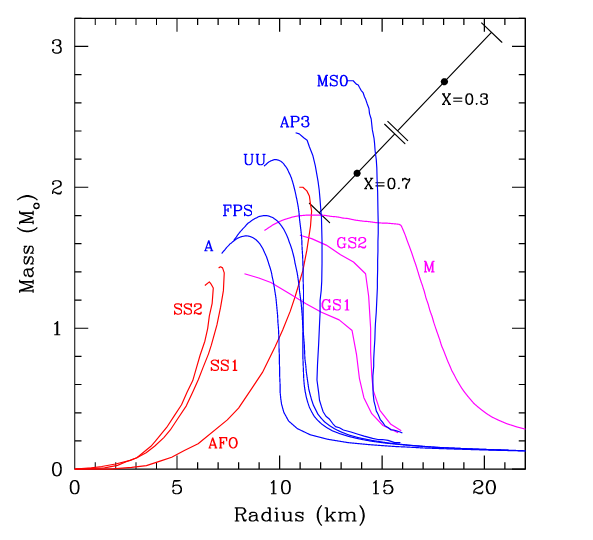
\includegraphics[width=0.75\textwidth]{ozel.png}
    \caption{The constraints on the neutron star equations of state imposed by observations of EXO 0748-676 from \cite{ozel2006}. Shown here are representative EOS for neutron stars without condensates (blue), with condensates (magenta), and for strange stars (red). The error bars on the points correspond to the uncertainty in the mass and radius as derived by \cite{ozel2006}. Two points are shown from Ozel's calculations: one with a hydrogen mass fraction of 0.7, which corresponds to the minimum allowed values for the mass and radius of the neutron star, and one with a hydrogen mass fraction of 0.3, which does not intersect with any of the displayed models.}
    \label{fig:ozel}
\end{figure}


\subsection{Discussion}

Ozel justifies the assumption that the entire star's surface is involved in the thermonuclear flash by the fact that the characteristic deflagration time\footnote{The deflagration time is the amount of time it takes for the combustion to propagate through all layers.} is less than one second, and that the magnetic field strength of this particular star is too weak to trap material in any one location. As long as these criteria are met, it is reasonable to assume that the burst is uniform across the entire star. It is argued in \cite{strohmayer1997} that the burst rise is non-uniform and exhibits millisecond oscillations, but these occur over only a 0.5 s interval of time and can be approximated as a uniform expansion on larger timescales. Additional observational evidence indicates that the peak luminosity of many bursts from the same star are self-consistent within 1\% \citep{galloway2003}, indicating that the entire surface of the neutron star emits uniformly during the burst phase. During the cooling phase, the observable $F_{cool}/T_c^4$ exhibits asymptotic behavior toward a constant (and consistent) value between bursts \citep{damen1990}. Ozel cites this as sufficient evidence to claim that emission remains uniform during the cooling phase as well, though there are low amplitude oscillations present that give rise to uncertainties smaller than the systematic and statistical uncertainties allowed in these calculations. \textbf{Furthermore, the photospheric radius expansion phase is the most important for constraining the neutron star mass and radius. There have not been any observations of flux oscillations during this phase, so this does not affect the determination of the Eddington limit from observations.} In addition, uncertainties related to magnetic and centrifugal effects are small, since EXO 0748-676 rotates slowly and has a low magnetic field.

In summary, the results of this study are highly significant for this star, but it remains to be seen whether this object is typical or not.

\subsection{Personal Relevance}

Ozel discusses a special type of thermonuclear X-ray burst that is strong enough to lift up the outer layers of the star. These photospheric radius expansion bursts are the exact phenomenon I simulate in my own research. The findings reported in this paper are that the equation of state of the interior has been determined using concurrent observations of multiple phenomena from a single source. If I hope to draw parallels between my simulations and observations that have been made by others, these kinds of results are highly valuable and can help constrain any models I construct. Additionally, it is useful for me to see this union between observation and theory to understand how results from my models could be either confirmed or ruled out by careful studies of individual stars.

The simulations I intend to run will also test some of the underlying assumptions of Ozel's analysis. For example, using the models I will construct, I will be able to examine the accuracy of the standard interpretation that the flux at the touch down point is equal to the Eddington flux---a crucial point for this observational work. More advanced analysis could provide insight into the accuracy of the spherically symmetric approximation, since it is already suspected that low-amplitude oscillations and the presence of magnetic fields could lead to a non-uniform burst. These simplifying assumptions tend to hold for this star in particular, since the magnetic field is weak and the timescale of the burst is so rapid. However, if one wishes to generalize the method to other stars, a higher level of precision may be required to account for the possibility of a non-uniform burst.

\bibliography{bibliography}{}
\bibliographystyle{aasjournal}

\end{document}

% End of file `sample63.tex'.
